\chapter{Revisão Bibliográfica} \label{cap2}

\section{Fundamentação Teórica}

\subsection{Estabilidade no sentido \textit{Lyapunov}}

% Introdução do teorema de Lyapunov
Os métodos de análise de estabilidade desenvolvidos por \textit{Lyapunov} são geralmente reconhecidos como base para a compreensão da estabilidade em sistemas dinâmicos. No ano de 1892, o matemático e engenheiro russo, \textit{Aleksandr Mikhailovich Lyapunov} (1857-1917), propôs abordagens que desempenham um papel crucial na compreensão e caracterização da estabilidade dos sistemas no ponto de equilíbrio. \cite{lyapunov1892}. Em essência, ela se concentra na análise do comportamento das soluções de sistemas dinâmicos em torno de pontos de equilíbrio, estabelecendo critérios para determinar a estabilidade desses pontos, sejam eles estáveis, instáveis ou assintoticamente estáveis. Desta forma, oferece métodos sistemáticos para avaliar a estabilidade de sistemas, tanto autônomos quanto não autônomos, abrangendo desde sistemas lineares até não lineares. \cite{khalil2002}. Ao fornecer condições suficientes para a estabilidade, os métodos de \textit{Lyapunov} oferecem uma estrutura poderosa para analisar e projetar sistemas dinâmicos com garantias de estabilidade desejadas.

% Bases para o teorema de Lyapunov
Considere o sistema dinâmico representado por \begin{equation}\dot{x} = f(x), \end{equation} onde $f: D \rightarrow \mathbb{R}^n$ é um mapeamento local \textit{Lipschitz} do domínio $D \subset \mathbb{R}^n$ em $\mathbb{R}^n$, e assuma que $\bar{x} \in D$ seja o ponto de equilíbrio do sistema, ou seja, $f(\bar{x}) = 0$. Dada a capacidade de transladar qualquer ponto de equilíbrio para a origem através de mudanças de variáveis, podemos, sem perda de generalização, definir a estabilidade do sistema em relação ao ponto de equilíbrio na origem, ou seja, $\bar{x} = 0$. Assim, podemos apresentar a definição da estabilidade do ponto de equilíbrio, conforme Khalil. \cite{khalil2002}.

\begin{definition}
  O ponto de equilíbrio $\bar{x} = 0$ é

  \begin{enumerate}
    \item[$\bullet$] estável se, para cada $\epsilon > 0$, existe $\delta = \delta(\epsilon) > 0$, tal que,
          $$ \lVert x(0)\rVert < \delta \Rightarrow \lVert x(t)\rVert < \epsilon, \hspace{0.3cm} \forall \, t \geq 0$$
    \item[$\bullet$] instável, se não for estável.
    \item[$\bullet$] assintoticamente estável, se for estável e $\delta$ possa   ser escolhido de forma que:
          $$ \lVert x(0)\rVert < \delta \Rightarrow \lim_{t \rightarrow \infty}x(t) = 0$$
  \end{enumerate}
\end{definition}

Portanto, para demostrar que o ponto de equilíbrio $\bar{x} = 0$ é estável, para qualquer valor de $\epsilon$, deve-se obter um valor de $\delta$, possivelmente dependente de $\epsilon$, de modo que uma trajetória que comece em uma vizinhança $\delta$ da origem nunca sairá da vizinhança $\epsilon$. \cite{khalil2002}.

Khalil, em seu livro \textit{Nonlinear Systems}, demonstrou que a estabilidade do ponto de equilíbrio de um sistema de pêndulo pode ser compreendida através do uso de conceitos de energia. Ele definiu a energia do pêndulo como a soma de suas energias potencial e cinética, com a escolha da referência da energia potencial de modo que a energia do pêndulo na origem seja nula. Ao desconsiderar o atrito, tornando o sistema conservativo e, consequentemente, mantendo a energia do sistema constante, observou-se a formação de um contorno fechado em torno do ponto de origem, especialmente para pequenos valores de energia do sistema. Assim, o ponto de origem é identificado como um ponto de equilíbrio estável. Para sistemas dissipativos, nos quais a energia do sistema diminui ao longo do tempo, ele observou que o sistema converge para a origem conforme o tempo tende ao infinito. Portanto, é possível determinar a estabilidade do ponto de equilíbrio analisando a derivada da função energia ao longo das trajetórias do sistema. \cite{khalil2002}.

Em 1892, Lyapunov afirmou que outras funções, além da energia, podem ser utilizadas para determinar a estabilidade do ponto de equilíbrio. \cite{lyapunov1892}. Dado $V : D \rightarrow \mathbb{R}$ uma função contínua diferenciável definida no domínio $D \subset \mathbb{R}^n$ que contém o ponto de origem. A derivada da função $V$ ao longo da trajetória de $f(x)$, denotado por $\dot{V}(x)$, demostrada por Khalil, \cite{khalil2002}, é dada por: \begin{equation} \dot{V}(x) = \frac{\partial V}{\partial x}f(x). \end{equation} Se $\phi(t;x)$ é a solução de $f(x)$ que inicia no estado inicial $x$ no tempo $t = 0$, então: \begin{equation} \dot{V}(x) = \left. \frac{d}{dt}f(\phi(t;x))\right|_{t=0}. \end{equation} Portanto, se $\dot{V}(x)$ é negativo, $V$ decresce ao longo da solução de $f(x)$.

% Esta é um boa forma de apresentar o teorema?
Com base nos conceitos apresentados até o momento, o teorema de estabilidade de Lyapunov pode ser definido como:

\begin{theorem}
  Seja $x = 0$ o ponto de equilíbrio para f(x) e seja $D \subset \mathbb{R}^n$ um domínio contendo $x = 0$. Seja $V : D \rightarrow \mathbb{R}$ uma função diferenciável contínua tal que:
  \begin{gather}
    V(0) = 0 \quad \text{e} \quad V(x) > 0 \quad \mathrm{em} \quad D - \{0\} \label{eq:lyapunov1} \\
    \dot{V}(x) \leq 0 \quad \mathrm{em} \quad D - \{0\} \label{eq:lyapunov2}
  \end{gather}
  Então, $x=0$ é estável. Além disto, se
  \begin{equation}
    \dot{V}(x) < 0 \quad \mathrm{em} \quad D - \{0\} \label{eq:lyapunov3}
  \end{equation}
  então, $x=0$ é assintoticamente estável.
\end{theorem}

%  Definição das função de Lyapunov, superfície de Lyapunov, e função DP e SDP.
Uma função $V(x)$ é chamada de função de Lyapunov quando é contínua e diferenciável, satisfazendo as equações \eqref{eq:lyapunov1} e \eqref{eq:lyapunov2}. A superfície $V(x) = c$, para qualquer $c > 0$, é referida como superfície de Lyapunov. Se $V(x)$ atende à condição \eqref{eq:lyapunov2}, isto é, $V(0) = 0$ e $V(x) > 0$ para $x \neq 0$, ela é considerada definida positiva. No caso em que $V(x)$ satisfaz $V(x) \geq 0$ para $x \neq 0$, ela é denominada semidefinida positiva. Uma função $V(x)$ é classificada como definida negativa ou semidefinida negativa se $-V(a)$ é definida positiva ou semidefinida positiva, respectivamente. Se $V(x)$ não se enquadra em nenhum desses casos, é considerada indefinida. Com essa terminologia, o teorema de Lyapunov pode ser reformulado, indicando que a origem é estável se existe uma função $V(x)$ definida positiva, continuamente diferenciável, tal que $\dot{V}(x)$ seja semidefinida negativa. Além disso, a estabilidade assintótica é alcançada quando $\dot{V}(x)$ é definida negativa. \cite{khalil2002}.

%  Definição das Matrizes SDP E DP
Uma classe de funções escalares para as quais a determinação do sinal pode ser facilmente realizada é a classe das funções quadráticas, representadas por:

\begin{equation}
  V(x) = x^T P x = \sum_{i=1}^n \sum_{j=1}^n p_{ij} x_i x_j
  \label{eq:lyapunov4}
\end{equation}

\noindent onde $P$ é uma matriz real simétrica. Nesse caso, $V(x)$ é positiva definida ou positiva semidefinida se, e somente se, todos os autovalores de $P$ são positivos ou não negativos, o que ocorre se e somente se todos os menores principais de $P$ são positivos ou não negativos, respectivamente. Se $V(x) = x^T P x$ é positiva definida ou positiva semidefinida, dizemos que a matriz $P$ é positiva definida ou positiva semidefinida, representado por $P > 0$ ou $P \geq 0$, respectivamente. \cite{khalil2002}.

%  To-do: adicionar um conclusão e uma ponte para LMIs
\subsection{Desigualdades Matriciais Lineares}

% Introdução às LMIs
As desigualdades matriciais lineares (\acrshortpl{lmi}, do inglês \textit{Linear Matrix Inequalities}) são de grande importância na teoria de controle e sistemas, fornecendo uma estrutura significativa para a formulação e resolução de uma variedade de problemas. Este conjunto de técnicas permite a representação de restrições complexas em termos de desigualdades lineares entre matrizes, possibilitando a abordagem de questões como estabilidade, desempenho e síntese de controladores de forma unificada. \cite{boyd1994}.

Os métodos de Lyapunov tradicionalmente empregados na análise de estabilidade de sistemas dinâmicos têm sido estendidos para permitir a formulação de \acrshortpl{lmi}, proporcionando assim uma base teórica sólida para a resolução de problemas de otimização e controle. Essa conexão entre \acrshortpl{lmi} e Lyapunov não apenas simplifica a análise e a síntese de sistemas complexos, mas também oferece uma estrutura matemática para abordar uma variedade de questões de controle de forma eficiente e sistemática. \cite{boyd1994}.

% História das LMIs
Como discutido na seção anterior, Lyapunov introduziu seus teoremas, estabelecendo que um sistema dinâmico \begin{equation} \dot{x}(t) = Ax(t) \label{eq:sys1}\end{equation} é assintoticamente estável se, e somente se, as condições descritas nas equações \eqref{eq:lyapunov1} e \eqref{eq:lyapunov3} forem satisfeitas. Adicionalmente, ele propôs uma classe de funções de Lyapunov que atendem a essas condições, conforme apresentado na equação \eqref{eq:lyapunov4}. Substituindo esta equação nas condições de estabilidade, obtemos: \begin{equation} \dot{V}(x) = \dot{x}^TPx + x^TP\dot{x} \label{eq:lyapunov5}. \end{equation} A partir do sistema (\ref{eq:sys1}), a equação (\ref{eq:lyapunov5}) pode ser reescrita como: \begin{equation} \dot{V}(x) = x^TA^TPx + x^TPAx \label{eq:lyapunov6}. \end{equation} logo, \begin{equation} \dot{V}(x) = x^T (A^TP + PA) x \label{eq:lyapunov6}, \end{equation} ou seja, o sistema (\ref{eq:sys1}) é assintoticamente estável se, e somente se, existir uma matriz definida positiva $P$ tal que \begin{equation} A^T P + P A < 0.\end{equation}

Essa condição, conhecida como desigualdade de Lyapunov em $P$, é uma forma específica de \acrshort{lmi}. Lyapunov também demonstrou que essa LMI inicial poderia ser resolvida explicitamente. Na prática, é possível escolher qualquer $Q = Q^T > 0$ e resolver a equação linear $A^T P + P A = -Q$ para a matriz $P$. Se o sistema for estável, a matriz $P$ resultante será definida positiva. Assim, a desigualdade de Lyapunov foi a primeira \acrshort{lmi} utilizada para analisar a estabilidade de sistemas dinâmicos, oferecendo uma solução analítica por meio da resolução de um conjunto de equações lineares. \cite{lyapunov1892,boyd1994}.

Após os trabalhos iniciais de Lyapunov, na década de 1940, pesquisadores soviéticos como Lur'e e Postnikov aplicaram seus métodos em problemas práticos de controle, focando especialmente na estabilidade de sistemas com não-linearidades nos atuadores. Embora suas soluções fossem resolvidas manualmente e aplicáveis apenas a sistemas menores, esse trabalho foi crucial para demonstrar a viabilidade das ideias de Lyapunov na engenharia de controle. O avanço seguinte, nos anos 1960, trouxe métodos gráficos mais acessíveis, expandindo o alcance para sistemas mais complexos e estabelecendo as bases para a resolução computacional das LMIs, marcando assim uma nova fase na teoria do controle. \cite{boyd1994}.

% Definição de um LMI
A seguir, é apresentado o conceito formal de uma \acrshort{lmi}, conforme definido por Boyd et al. \cite{boyd1994}.

\begin{definition}
  Uma \acrshort{lmi} é expressa pela equação \begin{equation} F(x) \triangleq F_0 + \sum_{i=0}^{m}(x_iF_i) > 0 \label{eq:lmi1}\end{equation} onde $x \in \mathbb{R}^m$ é a variável e as matrizes simétricas $F_i \in \mathbb{R}^{n \times n}, \, i = 0, . . . , m$, são fornecidas. Nesta expressão, o símbolo de desigualdade indica que $F(x)$ é definida positiva. Além disso, há \acrshortpl{lmi} não estritas, representadas pela forma \begin{equation} F(x) \geq 0 \end{equation}
\end{definition}

Múltiplas \acrshortpl{lmi}  $F_{(1)}(x) > 0, \, ..., \, F_{(p)}(x) > 0$ podem ser expressas como uma única \acrshort{lmi} $\mathbf{diag}(F_{(1)}(x), \, ..., \, F_{(p)}(x)) > 0$. Além disto, quando as matrizes $F_i$ são diagonais, a LMI $F(x) > 0$ é apenas um conjunto de desigualdades lineares. As desigualdades não lineares (convexas) são convertidas para a forma LMI usando complementos de Schur.

A \acrshort{lmi} \eqref{eq:lmi1} é uma restrição convexa em $x$, tornando o conjunto $\{x \, : \, F(x) > 0\}$ convexo e pode representar uma ampla variedade de restrições convexas em $x$, incluindo desigualdades lineares, quadráticas, de norma de matriz, bem como restrições comuns em teoria de controle, como desigualdades matriciais quadráticas convexas e de Lyapunov. \cite{boyd1994}.

\subsection{Sistemas de Controle Baseado em Eventos}

% ETC: Introdução
O \acrfull{etc}, surgindo como uma solução, se destaca em \acrfullpl{scr}, onde conectam componentes como sensores, controladores e atuadores através de uma rede compartilhada. Enquanto os \acrshortpl{scr} geralmente adotam o controle periódico, o que pode causar congestionamentos e desperdícios de recursos, o \acrshort{etc} executa tarefas apenas quando necessárias, minimizando estes problemas. Ele pode ser modelado de diversas formas, com destaque para o modelo de atraso de tempo, que permite lidar com atrasos de transmissão e otimizar ganhos de controle. Esses modelos despertam interesse entre pesquisadores, especialmente em estudos de estabilidade e design de controladores \cite{peng2018}.

O modelo de um sistema dinâmico em loop fechado com um \acrshort{etc} implementado pode ser descrito como um modelo típico de controle de feedback de estado, conforme ilustrado na figura a seguir.

\begin{figure}[H]
  \centering
  % \vspace{3ex}
  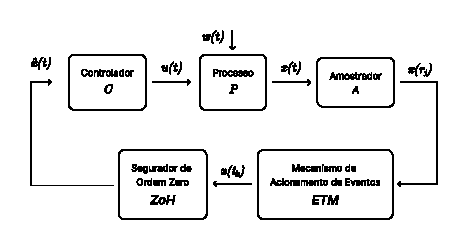
\includegraphics[scale=2.]{figuras/etc-model.eps}
  \caption{Modelo de um sistema dinâmico em loop fechado com ETC.}
  \label{fig:etc-model}
\end{figure}

% ETC: Estrutura
O modelo apresentado na \autoref{fig:etc-model} consiste em uma planta $ P$ que recebe uma entrada de perturbação não controlada $w(t)$ e a entrada de controle $u(t)$, e cujo estado é determinado por uma equação diferencial \begin{equation}\dot{x}(t) = f(x(t), u(t), w(t))\end{equation} A informação do estado pode ser monitorada de forma contínua ou amostrada, o que caracteriza o \acrshort{etc} como contínuo ou periódico, respectivamente. No caso do \acrshort{etc} periódico, um sistema de amostragem é introduzido para gerar uma sequência discreta de estados $x(t_A)$, onde o $t_A$ é o tempo de liberação do estado medido. Por outro lado, no \acrshort{etc} contínuo, o estado medido é enviado diretamente para o \acrshort{etm}. \cite{peng2018,coutinho2021,Lemmon2010}.

% ETC: Função do ETM e comportamento Zeno
O \acrshort{etm} determina o instante apropriado para transmitir o estado para o \acrfull{zoh} - que é utilizado para transformar o sinal discreto resultante em um sinal contínuo no tempo,  para estar disponível para o controlador $C$ que irá mapear esses estados amostrados em um sinal de controle e aplicar à planta. \cite{coutinho2021}. Para garantir a eficácia do \acrshort{etm}, é crucial evitar o comportamento Zeno. Esse comportamento ocorre quando o controlador executa uma quantidade infinita de tarefas de controle dentro de um intervalo de tempo finito, contrariando a premissa fundamental do \acrshort{etc} de minimizar os tempos de execução de tarefas. Além disso, o fenômeno de Zeno exerce uma considerável influência nos comportamentos dinâmicos dos sistemas, manifestando-se em instabilidade, degradação de desempenho e oscilações indesejadas. \cite{Yang2024}.

% ETC: Diferentes Abordagens - Introdução e Abordagem por Emulação
O projeto eficiente tanto do \acrshort{etm} quanto das leis de controle é crucial para assegurar o desempenho adequado e a estabilidade dos sistemas \acrshort{etc} em malha fechada. Como resultado, os modelos de \acrshort{etc} frequentemente adotam abordagens baseadas em emulação ou co-design para atingir tais objetivos. \cite{coutinho2021, peng2018}. As abordagens baseadas em emulação são geralmente realizadas em dois passos distintos. Primeiramente, um controlador é projetado para garantir a estabilidade ou um desempenho específico para o sistema em malha fechada, assumindo a ausência do \acrshort{etm} e da rede de comunicação. Este controle é projetado de acordo com uma estrutura convencional de dados amostrados periódicos, aproveitando os resultados proveitosos dos sistemas de dados amostrados. \cite{coutinho2021,peng2018}. Em seguida, o segundo passo envolve a consideração da presença do \acrshort{etm} e dos efeitos induzidos pela rede de comunicação, a fim de projetar o \acrshort{etm} de forma a preservar as propriedades garantidas pelo controlador previamente projetado. Esta abordagem permite que o \acrshort{etm} seja projetado separadamente do controle, conferindo flexibilidade no processo de projeto. \cite{coutinho2021,peng2018}. No entanto, essa independência pode limitar o desempenho em malha fechada do sistema \acrshort{etc} e exigir mais transmissões do que o necessário, uma vez que o \acrshort{etm} pode não estar otimizado para o controle específico. \cite{coutinho2021}.

% ETC: Diferentes Abordagens - Abordagem por Co-design
As abordagens baseados no \textit{co-design} buscam superar as limitações das abordagens baseadas em emulação, permitindo o design simultâneo do \acrshort{etm} e da lei de controle. No entanto, o \textit{co-design} enfrenta desafios como problemas de otimização não-convexos ou multiobjetivo, devido a restrições conflitantes de desempenho e aumento dos tempos entre eventos. A análise muitas vezes se limita a classes específicas de controladores e \acrshortpl{etm} \cite{coutinho2021}. Diferentes estratégias de \textit{co-design} têm sido desenvolvidas para várias formas de \acrshortpl{etm}. Estas incluem \textit{co-design} estático para estabilização local de sistemas LTI e \textit{co-design} dinâmico para sistemas lineares com entradas não lineares limitadas, entre outros. As condições de \textit{co-design} são frequentemente derivadas usando formalismos de sistema híbrido e expressas em termos de \acrshortpl{lmi}, permitindo uma eficiente resolução por métodos de otimização convexa \cite{coutinho2021}.

% ETC: ETM estático e dinâmico (adaptativa)
Os modelos de \acrshort{etm} podem ser diferenciados em termos da lei de acionamento, que pode ser estática ou adaptativa (dinâmica). No contexto do \acrshort{etm} estático, os instantes de transmissão são determinados com base em uma função de acionamento estática. Destaca-se, a título de ilustração, o \acrshort{etc} contínuo estático proposto por Tabuada \cite{Tabuada2007}, esclarecendo sua eficácia para sistemas não lineares em malha fechada, onde a estabilidade é garantida por meio de uma função \acrfull{ees} de \textit{Lyapunov}.

Para reduzir o número de eventos transmitidos, foram propostas funções de acionamento aprimoradas \cite{Wang2020,Zong2023,Ge2017, Ning2018, Wu2021}, introduzindo variáveis dinâmicas. Uma alternativa é considerar uma função de ponderação variável no tempo, caracterizando o \acrshort{etc} adaptativo ou dinâmico, desenvolvido principalmente no contexto de sistemas \acrshort{etc} periódico \cite{coutinho2021}. Este método permite ajustar dinamicamente o limite de acionamento, proporcionando uma adaptação mais flexível às condições do sistema. A estabilidade do sistema sob o \acrshort{etc} adaptativo é analisada usando uma função de \textit{Lyapunov} modificada, demonstrando sua eficácia em manter a estabilidade em malha fechada \cite{coutinho2021}.

% ETC: Rede de Comunicação
Os efeitos induzidos aos estados transmitidos pela rede de comunicação $\mathcal{N}$ são de suma importância e têm um impacto direto na estabilidade e no desempenho do sistema. Quando os estados são transmitidos por meio da rede, podem surgir distorções e atrasos devido a vários fatores, como variações nos intervalos de transmissão, atrasos na própria rede e possíveis perdas de pacotes. Essas perturbações nos estados transmitidos podem resultar em erros na estimativa do estado real no controlador, afetando diretamente a capacidade do sistema de alcançar os objetivos de controle desejados. Assim, é essencial compreender e mitigar esses efeitos nos estados transmitidos para garantir um projeto eficaz dos controladores, o que por sua vez assegura a estabilidade e o desempenho adequados do sistema em malha fechada. \cite{coutinho2021}.

% ETC: Conclusão
As diferentes abordagem de \acrshort{etc} abrangem investigações em controladores de retroalimentação de estado, observadores, \acrshortpl{etm} estáticos e dinâmicos, com o intuito de assegurar a estabilidade e o desempenho em malha fechada em uma variedade de sistemas, tais como sistemas \acrfullpl{lit} \cite{Zong2023,Wu2021}, sistemas de \textit{Lur'e} \cite{Zhang2017} e modelos \textit{fuzzy Takagi-Sugeno} \cite{Pan2017}. O foco está em estabelecer condições práticas e numericamente solucionáveis que simplifiquem o projeto eficaz de sistemas de controle complexos.

% ---------------------------------------------------------------------------
\section{\acrshort{etm} Dinâmico e Estático}

% ETM: Apresentação do trabalho de Coutinho
Em sua pesquisa, Coutinho investigou um modelo de \acrshort{etm} dinâmico e estático, sobre o qual este projeto se fundamenta. Este modelo baseia-se em uma condição suficiente para permitir o projeto simultâneo do \acrshort{etm} e do controlador com ganhos escalonados, por meio da abordagem por co-design, garantindo a estabilidade assintótica da origem do sistema em malha fechada. Além disso, ele provou a existência de um \acrfull{imee} positivo que evita a existência de comportamento de Zeno a fim de garantir sua aplicabilidade, pois as redes de comunicação não têm largura de banda infinita para suportar tempos entre eventos arbitrariamente próximos. Por fim, aborda um problema de otimização visando a ampliação dos intervalos entre eventos, com o objetivo de minimizar a quantidade de eventos gerados pelo \acrshort{etm}. \cite{coutinho2021}.

% ETM: Apresentação do sistema dinâmico
O modelo proposto por Coutinho para o \acrshort{etm} dinâmico considera uma classe específica de sistemas não lineares, representada pela equação diferencial abaixo: \begin{equation} \dot{x}(t) = A(x(t))x(t) + B(x(t))u(t). \label{eq:etm-sys}\end{equation} Nesta equação, $ x(t) \in D \subset \mathbb{R}^n $ representa o estado do sistema, $ u(t) \in \mathbb{R}^m $ é a entrada de controle, e $ A: D \rightarrow \mathbb{R}^{n \times n} $ e $ B: D \rightarrow \mathbb{R}^{n \times m} $ são funções contínuas de matriz, com a restrição de que $ B(x) \neq 0 $ para todo $ x \in D $. Os termos não lineares nos coeficientes dependentes do estado, $ A(x) $ e $ B(x) $, são representados por $ z_j: D \rightarrow \mathbb{R} $, onde $ j \in \mathbb{N}_{\leq p} $, e são denominados funções de escalonamento. Aqui, $ D \subset \mathbb{R}^n $ é um politopo convexo que inclui a origem, sendo esta considerada o ponto de equilíbrio de interesse. \cite{coutinho2021}.

% Definição das funções de escalonamento e de ponderamento
% Warning Este texto é praticamente igual a do Coutinho
Dado que as funções de escalonamento $z_j(x)$ são contínuas e $D$ é um conjunto compacto, podemos inferir a existência de limites, de forma que: \begin{equation} z_{j}^0 \leq z_j(x) \leq z_{j}^0, \quad \forall j \in \mathbb{N}_{\leq p}. \end{equation} Assim, cada função de escalonamento $z_j(x)$ pode ser representada de maneira equivalente como: \begin{equation} z_j(x) = w_0^j(x)z_j^0 + w_{1}^j(x)z_{j}^1 = \sum_{i_j=0}^{1} w_{i_j}^j(x)z_i^{i_j}, \end{equation} onde as funções de ponderação dependentes do estado são definidas como: \begin{equation} w_0^j(x) := \frac{z_j^1 - z_j(x)}{z_j^1 - z_j^0}, \quad w_1^j(x) := 1 - w_0^j(x), \end{equation} com $0 \leq w_i^j(x) \leq 1$, $i_j \in \mathbb{B}$, $j \in \mathbb{N}_{\leq p}$. Portanto, para todo $x \in D$, o sistema não linear \eqref{eq:etm-sys} pode ser equivalente ao seguinte modelo quasi-LPV poliédrico: \begin{equation} \dot{x}(t) = \sum_{i \in \mathbb{B}_p} w_i(x(t))(A_i x(t) + B_i u(t)), \label{eq:etm-politopic} \end{equation} onde os parâmetros dependentes do estado são definidos como: \begin{equation} w_i(x) := \prod_{j=1}^{p} w_{ij}^j(x), \end{equation} sendo $i = (i_1, ..., i_p) \in \mathbb{B}_p$. Por definição, observamos que a propriedade de soma convexa permanece válida para os parâmetros: \begin{equation} \sum_{i \in \mathbb{B}_p} w_i(x) = 1, \quad 0 \leq w_i(x) \leq 1, \quad \forall i \in \mathbb{B}_p, \end{equation} garantindo que as matrizes: \begin{equation} \left. A_i := A(x) \right|_{w_i(x)=1}, \quad \left.B_i := B(x) \right|_{w_i(x)=1}, \end{equation} definem os vértices do modelo quasi-LPV poliédrico \eqref{eq:etm-politopic}. \cite{coutinho2021}.

% ETM: Lei de controle 
A seguinte lei de controle de realimentação de estado, com ganhos escalonados, é considerada para estabilizar o sistema \eqref{eq:etm-sys}:
\begin{equation} u(t) = K(\hat{x}(t))\hat{x}(t) = \sum_{j \in Bp} w_j(\hat{x}(t))K_j\hat{x}(t) \end{equation} onde $ \hat{x}(t) $ representa a informação de estado disponível para o controlador através do ETM. A matriz dependente de estado $ K : D \rightarrow \mathbb{R}^{m \times n} $ é assumida como dependente das funções de escalonamento de \eqref{eq:etm-sys}, de modo que um controlador programado para ganho com ganhos $ K_j = K(\hat{x}) $ possa ser parametrizado em termos dos parâmetros $ w_j(\hat{x}) $. \cite{coutinho2021}.

% ETM: Apresentação do erro de transmissão
Quando uma amostra de dados é transmitida no tempo do evento $t_k$, o estado disponível para o controlador é atualizado para $\hat{x}(t) = x(t_k)$, para todo $t \in [t_k, t_{k+1})$. Como é utilizado um \acrshort{zoh}, $\hat{x}(t)$ é mantido constante até o próximo tempo de evento $t_{k+1}$, o que induz o erro de transmissão \begin{equation}e(t) = \hat{x}(t) - x(t) \label{eq:etm-error},\end{equation} $\forall t \in [t_k, t_{k+1})$. \cite{coutinho2021}.

% ETM: Tempo de ocorrência dos eventos e a variável interna dinâmica
O tempo de ocorrência dos eventos é determinado pela seguinte equação: \begin{equation} t_0 = 0, t_{k+1} = \inf \{t > t_k : \eta(t) + \theta \Gamma(x(t), e(t) < 0) \}, \, \forall k \in \mathbb{N}, \end{equation} onde $\theta \in \mathbb{R}_{\geq 0}$ é um parâmetro de projeto e a função de acionamento $\Gamma(x, e)$ é definida como: \begin{equation} \label{eq:etm-gama} \Gamma(x, e) = x^T \Psi x - e^T \Xi e - \zeta (x,e), \end{equation} com \begin{equation} \zeta(x, e) = 2x^TPB(x)(K(\hat{x}) - K(x))(x+e). \end{equation} A dinâmica da variável interna do \acrshort{etm} é definida como: \begin{equation}  \dot{\eta} = - \lambda \eta(t) + \Gamma(x(t), e(t)), \end{equation} onde $\lambda \in R_{\geq} 0 $ é o parâmetro de projeto relacionado à taxa de decaimento de $\eta(t)$. \cite{coutinho2021}.

% ETM: Condições de Co-design

A condição suficiente proposta para projeto por co-design para o ETC contínuo  e o controlador por ganhos escalonados é declarada a seguir.
\begin{theorem}
  \label{theorem:constraints-2}
  Dados $\theta, \eta_0 \in \mathbb{R}_{\geq 0}$, e $\lambda \in \mathbb{R}_{> 0}$, se existirem as matrizes $\tilde{K}_j \in \mathbb{R}^{m \times n}, j \in B_p$. e matrizes simétricas positivas definidas $\Xi, \Psi, X \in \mathbb{R}$, satisfazendo as seguintes \acrshortpl{lmi}:
  \begin{equation}
    \sum_{(\mathbf{i}, \mathbf{j}) \in \mathscr{P} (\mathbf{m},\mathbf{n})} \Upsilon_{\mathbf{ij}} < 0, \quad \forall \mathbf{m}, \mathbf{n} \in B_p^+,
    \label{eq:2.18}
  \end{equation}
  onde
  \begin{equation}
    \Upsilon_{\mathbf{ij}} :=
    \begin{bmatrix}
      He(A_\mathbf{i}X +B_\mathbf{i}\tilde{K}_\mathbf{j}) & B_\mathbf{i}\tilde{K}_{\mathbf{j}} & X             \\
      \star                                               & -\tilde{\Xi}                       & 0             \\
      \star                                               & \star                              & -\tilde{\Psi}
    \end{bmatrix},
  \end{equation}
  então, a origem do sistema de malha fechada é assintoticamente estável com $K_j = \tilde{K}_jX^{-1}$, $j \in B^p$, $\Xi= X^{-1}\tilde{\Xi}X$, $\Psi = \tilde{\Psi}^{-1}$, $P = X^{-1}$ e função de Lyapunov
  \begin{equation}
    W(x, \eta) = V(x) + \eta,
  \end{equation}
  com $V(x)=x^TPx$.
\end{theorem}

Para reduzir o número de eventos gerados, Coutinho propôs o seguinte problema de otimização convexa que visa minimizar $\lambda_{\max} (\Xi)$ e maximizar $\lambda_{\min}(\Psi)$: \begin{equation}\underset{Q, X, \tilde{\Xi}, \tilde{\Psi}, \tilde{K}_\mathbf{j}}\min \quad \mathbf{tr}(\tilde{\Xi} + \tilde{\Psi} + Q).\end{equation} Este problema é sujeito a restrições apresentadas no \autoref{theorem:constraints-2} e à seguinte \acrshort{lmi} de restrição \begin{equation}\begin{bmatrix}
  -Q & I \\ \star & -X
\end{bmatrix} < 0.\end{equation} A solução deste problema tende a minimizar os autovalores de $Q$, $\tilde{\Xi}$ e $\tilde{\Psi}$ e a reduzir os tempos entre os eventos. \cite{coutinho2021}.

Ao considerar um valor de $\theta$ suficientemente grande, o \acrshort{etm} dinâmico converge para uma versão estática, que se torna completamente independente de $\eta(t)$, conforme descrito a seguir: \begin{equation} t_0 = 0, \quad t_{k+1} = \inf\{t > t_k : \Gamma(x, e) < 0\}, \forall k \in \mathbb{N}, \end{equation} onde $\Gamma(x, e)$ é definido em \eqref{eq:etm-gama}. \cite{coutinho2021}.

\section{Trabalhos Relacionados}

A área de sistemas \acrshort{etc} já possui diversas técnicas estabelecidas que têm demonstrado resultados promissores. As estratégias adotadas neste projeto têm sua base em pesquisas destacadas que serão apresentadas a seguir

% To-do: Explicar sobre o comportamento Zeno na fundamentação
% Dúvida: É para ser mais detalhistas em cada trabalho?
No estudo realizado por Coutinho \cite{coutinho2021}, é investigado o \textit{co-design} de controladores de retroalimentação de estado, e \acrshortpl{etm} contínuos e dinâmicos para sistemas comutados não lineares representados por modelos \textit{quasi} \acrfullpl{lpv}. A condição de \textit{co-design} é derivada com base na teoria da estabilidade de \textit{Lyapunov} para garantir a estabilidade assintótica do sistema \textit{Lyapunov} em malha fechada. Para lidar com o fenômeno assíncrono entre o controlador e os parâmetros do modelo \textit{quasi}-\acrshort{lpv} induzido pela ação do \acrshort{etm}, é proposta uma função de acionamento que cancela essa influência, resultando em uma condição de \textit{co-design} menos conservadora. Também é introduzido um problema de otimização convexa para aumentar os tempos entre eventos. Ademais, é demonstrada a existência de um \acrfull{imee} para o \textit{etc} contínuo proposto, evitando o comportamento \textit{Zeno}. Além disso, são apresentadas as vantagens da abordagem de \textit{co-design} dinâmico sobre a abordagem baseada em emulação e sua versão estática.

% Lembrete: Este trabalho apresenta a definição de zoh
% Dúvida: Há um termo melhor para 'switched systems'?
\textit{Ren et al}. \cite{Ren2018} abordaram o controle resiliente de tempo finito com base em observadores para sistemas comutados, realizado em um \acrfull{ecae}. Diferenciando-se dos problemas tradicionais de tempo finito, este estudo considera não apenas o \acrfull{ltf}, mas também a \acrfull{efes}. Um \acrshort{ecae} é formulado para sistemas comutados, visando uma utilização eficiente dos recursos da rede. Para lidar com a impossibilidade de medir todos os estados, é desenvolvido um observador acionado por eventos, que serve como base para a construção de um controlador resiliente. Esse controlador demonstra robustez ao estabilizar os sistemas em questão, dentro do contexto do controle de tempo finito. Utilizando o método de atraso no tempo e a abordagem de \textit{Lyapunov}, são derivados resultados significativos para avaliar as propriedades dos \acrshortpl{ltf} e da \acrshort{efes} dos sistemas de erro comutados em circuito fechado acionados por eventos. Todas as desigualdades matriciais são transformadas em \acrshortpl{lmi} para facilitar a obtenção conjunta dos ganhos do controlador e do observador. Por fim, a eficácia do esquema de controle proposto é demonstrada através de sua aplicação em um sistema de circuito de conversor \textit{boost}.

No estudo apresentado por \textit{Soni et al}. \cite{Soni2023}, é proposto o \acrshort{etc} para o modelo \acrshort{lpv} de conversores \textit{boost}. O controlador proposto, dependente da razão de ciclo, demonstra melhor desempenho e menor demanda computacional. Utilizando a função de \textit{Lyapunov } dependente de parâmetros, foi realizada a análise de estabilidade da abordagem proposta. Além disso, é estabelecido que o tempo entre eventos é limitado inferiormente por uma constante positiva, assegurando um desempenho livre de comportamento \textit{Zeno}. Os resultados de simulação e experimentais deste estudo validam a eficácia do método proposto, evidenciando que o modelo proporciona desempenho e maior robustez.

% Dúvida: Há um termo melhor para 'switched systems'?
No estudo realizado por Ma et al. \cite{Ma2016}, o problema do \acrshort{etc} com base em retroalimentação de saída para sistemas lineares comutados é investigado. Os autores projetam um controlador acionado por eventos e derivam condições suficientes para garantir a estabilidade assintótica do sistema comutado, utilizando métodos da função de \textit{Lyapunov} e técnicas de \acrshortpl{lmi}. Além disso, eles demonstram que o \acrshort{imee} acionados é positivo, eliminando o comportamento Zeno na amostragem. Por fim, os pesquisadores aplicam seu método a sistemas comutados de conversores \textit{boost} para validar sua eficácia.

\textit{Xie et al.} \cite{Xie2023} abordam os problemas da análise de \acrshort{efes} e do projeto de controlador de retroalimentação de saída para sistemas afins comutados sujeitos a perturbações externas. Um observador afim comutado é desenvolvido para estimar estados não mensuráveis, seguido pela proposição de um \acrshort{etm} dinâmico capaz de evitar o comportamento Zeno e reduz a carga de transmissão da rede. As condições viáveis da \acrshort{ees} são apresentadas em formas de \acrshortpl{lmi}, baseadas em uma função de \textit{Lyapunov-Krasovskii} temporal e leis de comutação dependentes do estado. A eficácia do algoritmo proposto é demonstrada através de um exemplo de aplicação com um conversor \textit{flyback} CC-CC.

No artigo \cite{Kumar2020}, Kumar et al. introduzem um novo conceito de \acrshort{etc} para otimizar o uso de recursos em \acrshort{mgcc}. Um \acrfull{cmd} é combinado com um observador de perturbações integral para suprimir incertezas combinadas e não combinadas em modo conectado à rede e isolado. O controlador resultante regula a tensão do barramento \acrshort{cc} e melhora a estabilidade operacional da \acrshort{mr}. Um \acrshort{cmd} convergente em tempo finito, livre de oscilações, é desenvolvido com uma lei de alcance de super torção para garantir robustez. A eficácia do \acrshort{etc} é comparada com abordagens alternativas e demonstrou um desempenho superior.
